\documentclass[a4paper]{article}

\usepackage[english]{babel}
\usepackage[UKenglish]{isodate}
\usepackage[parfill]{parskip}
\usepackage{algorithm}
\usepackage{algpseudocode}
\usepackage{float}
\usepackage{graphicx}
\usepackage{booktabs}
\usepackage{csquotes}
%\usepackage[margin=2.5cm]{geometry}
\usepackage{listings}
\usepackage{enumerate}
\usepackage{siunitx}
\usepackage{amssymb}
\usepackage{amsthm}
\usepackage{mathtools}
\usepackage{appendix}
\usepackage[style=ieee,
            natbib=true,
            backend=biber]{biblatex}

\addbibresource{references.bib}
\usepackage[hidelinks]{hyperref}
\nocite{*}

\DeclarePairedDelimiter{\ceil}{\lceil}{\rceil}
\DeclarePairedDelimiter{\floor}{\lfloor}{\rfloor}

\newcommand\ddfrac[2]{\frac{\displaystyle #1}{\displaystyle #2}}

\newcommand{\nth}{\textsuperscript}
\renewcommand*{\arraystretch}{1.3}

\newtheorem*{lemma}{Lemma}
\newtheorem*{theorem}{Theorem}

\title{Modifying Markov Chains to Model Traffic Jams}
\author{Kevin Zihong Ni\\\texttt{z5025098}}

\begin{document}

\maketitle

\begin{abstract}
	In this paper, we will describe the modification and adaptation of a traditional discrete time Markov Chain to efficiently model how 
	traffic jams evolve based on the live traffic conditions of every road in a network.
	We will show how this model performed experimentally with respect to both accuracy and time.
	We also will identify limitations in the model and techniques to mitigate them.
\end{abstract}

\section{Introduction}
Vehichular route planning is an important service in the software industry, being provided by various companies such as Google, Apple and Uber.
Some of these services collect live traffic data through the gps units in the smartphones of drivers.
This data is used to improve route planning, choosing routes to avoid high traffic areas.
However, traffic conditions in a road network changes over time and areas that are currently experiencing high traffic may clear up over the next minutes and vice versa.
This is problematic for route planning over long distances, 
as an algorithm may produce a route that goes around an existing traffic jam which would have cleared by the time the driver had reached it.  
It is apparent how traffic forecasting systems could be of benefit to these routing algorithms.

While it is possible to predict, with relative accuracy, the conditions of roads based on historical data, 
these models break down in abnormal traffic conditions that may be caused by external events such as accidents or roadworks.
The model this paper explores uses a combination of historical and live traffic data in order to make short to medium term forecasts that take into account any 
abnormal conditions. 

\section{Model}
While the behaviour of individual cars on the street are highly unpredictable (without the knowledge of its intended destination), we notice that the collective behaviour 
of all cars in a road network becomes very predictable.
By this, we mean that the traffic conditions of the entire network is highly dependent on the traffic conditions of the network a few moments in the past.
This is an area which lends itself to Markov Chains well, as shown by previous uses of the technique such as modelling demographic shift.
Markov chains model the changes in the states between discrete timesteps. 
Hence, before we define our model, we must first declare how much real world time (in seconds) does one timestep represent. 
Let this timestep be $t$.

\subsection{Topology}
We assume we are given a set of roads $E$ and a set of intersections $V$ together making a directed graph $G = (V, E)$.
Every edge $e \in E$ also has a length $d(e)$ and a speed $s(e)$ associated with it.
For simplicity, we also assume that $G$ has no self loops or parallel edges. These features can be trivially added to the model if necessary.

We also make the reasonable assumption that $G$ is strongly connected.
This can be done as the alternative implies either one of the following statements:
\begin{itemize}
	\item There are more than one connected components in which case we can create a separate model for each component.
	\item There are more than one strongly connected components which implies that there are places in the network which 
		a vehichle can enter but never leave (or vice versa) which is clearly absurd.
\end{itemize}

The states of our Markov chain will simply be the set of edges $E$, since this is where the overwhelming majority of cars will be at any one time.

\subsubsection{Road Based Graph}
Since the vertices of the graph represented by a Markov Matrix will become the states of that respective Markov Chain, it is necessary to 
transform our intersection based graph $G$ into another, road based graph $G' = (E, T)$ as outlined by \cite{volk}. 
$T$ denotes the set of possible "turns" in $G$, i.e. the set of possible transitions from one road to another.
An example of this transformation is illustrated in figures \ref{fig:int} and \ref{fig:roa}.

\begin{figure}[h]
    \centering
    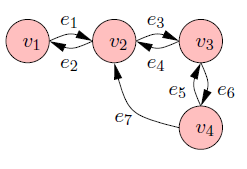
\includegraphics[width=0.4\textwidth]{intersection.PNG}
    \caption{intersection based graph}
    \label{fig:int}
\end{figure}

\begin{figure}[h]
    \centering
    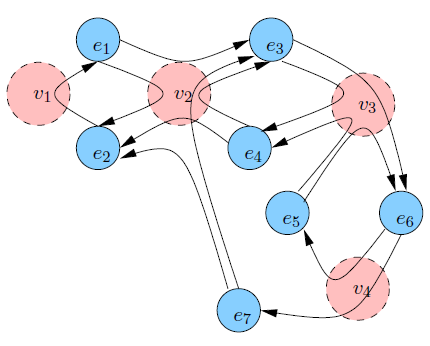
\includegraphics[width=0.7\textwidth]{road.PNG}
    \caption{road based graph}
    \label{fig:roa}
\end{figure}

\subsubsection{Turn Weights}
We also must assign a weight to each turn $t \in T$. 
This weight will be used as the (base) transition probability in the markov chain. 
When calculating these weights, we assume that their destinations has the capacity to accept an infinite number of cars. 
This number will be fixed to accomadate these road capacities later.
First, we will need to determine what fraction of cars in each road $e \in E$ will leave $e$ in each timestep. 
We define this to be
$$
l(e) = \min \left(1, \ddfrac{t \epsilon s(e)}{d(e)} \right)
$$

where $\epsilon$ is a constant that accounts for small losses in efficiency due to turning and unexpected changes in speed.

We now consider the edges that $e$ is connected to. The combined weights of all turns to these edges must total $l(e)$.
The simplest solution to this would be to just assign $l(e)/\mathrm{outdegree}(e)$ to each turn.
However, here we also have an opportunity to incorporate historical data into our model.
Provided we have the empirical data showing the number of different turns made at each likelihood 
(which should be trivial to implement with mobile phone live traffic collection), we can calculate the relative likelihood of a turn out of $e$ to each turn $e'$, $P(e, e')$.
The weight of the turn $(e, e')$ will then be $P(e, e') l(e)$.

Putting this all together, we can construct $T$ with the following algorithm
\begin{algorithmic}[1]
	\Function{FindTurns}{$G$}
		\State $T \gets \varnothing$
		\For{$v \in V$}
			\For{$e \in \mathrm{incoming}(v)$}
				\For{$'e \in \mathrm{outgoing}(v)$}
					\State $T \gets T \cup {(e, e', P(e, e') l(e)}$
				\EndFor
			\EndFor
		\EndFor
		\State return $T$
	\EndFunction
\end{algorithmic}

\subsection{State Transitions}

\printbibliography
\end{document}
